\section{Results}\label{sec:results}

\subsection{Replication of the base method}\label{sec:res-repl}

Our implementation of crisp RFM-FCA reproduces \citet{rungruang2024} on Online Retail II: 805,620 cleaned transaction lines, 5,878 customers and 208 formal concepts, as published. Over the 34 concept sizes printed in the paper the mean absolute difference is 0.8 customers (20 exact), and all 18 published association rules are recomputed with confidences within 0.01. Two reporting details had to be inferred: zero-price lines are kept (the published row count is reached only then), and recency is counted in calendar days.

\subsection{Method development and confirmation}\label{sec:res-dev}

The first fuzzy specification used sigma-count support. It was pre-registered on Online Retail II and failed: with fixed regularisation, the Łukasiewicz lattice (2,568--2,647 concepts per training fold) predicted worse than crisp RFM-FCA (AUC 0.733 vs 0.781, $R^2$ 0.173 vs 0.298), as Proposition~\ref{prop:floor} anticipates. Replacing it by core support reduces the segments to 208 on the full data. With fixed regularisation the core-filtered lattice was still slightly worse than the crisp one on Online Retail II (AUC $-0.007$), whereas with tuned regularisation it was better; tuned regularisation was therefore pre-specified for all later analyses.

The method was then tested unchanged on the two other datasets with seven pre-registered claims each. On CDNOW all seven replicated (Holm-adjusted $p = 0.005$ each): fuzzy memberships beat crisp scores, the fuzzy lattice beat the crisp lattice, the lattice added spend signal beyond the fuzzy memberships, and fuzzy representations changed less when transactions were dropped. On dunnhumby four replicated (memberships and lattice beating their crisp counterparts on both metrics) and three did not: the lattice predicted spend \emph{worse} than the fuzzy memberships ($R^2$ $-0.008$), and neither robustness claim held. These two findings are therefore not general, and we do not claim them.

\subsection{Prediction}\label{sec:res-pred}

\begin{table}[t]
\centering\small
\caption{Out-of-sample prediction of the next 90 days (means over four cutoffs; regularisation tuned by inner cross-validation). Best value per column in bold.}
\label{tab:prediction}
\begin{tabular}{lcccccc}
\toprule
 & \multicolumn{3}{c}{ROC AUC (purchase)} & \multicolumn{3}{c}{$R^2$ (log spend)} \\
\cmidrule(lr){2-4}\cmidrule(lr){5-7}
Representation & Retail II & CDNOW & dunnhumby & Retail II & CDNOW & dunnhumby \\
\midrule
Crisp scores (C-ctx) & 0.782 & 0.784 & 0.869 & 0.296 & 0.209 & 0.511 \\
Crisp RFM-FCA (C-fca) & 0.780 & 0.784 & 0.855 & 0.299 & 0.222 & 0.508 \\
Fuzzy memberships (F-ctx) & \textbf{0.787} & \textbf{0.789} & 0.877 & 0.304 & 0.219 & \textbf{0.525} \\
Fuzzy RFM-FCA (F-fca-core) & 0.786 & 0.788 & 0.865 & \textbf{0.308} & 0.235 & 0.517 \\
log-RFM & 0.786 & 0.788 & \textbf{0.887} & 0.293 & \textbf{0.241} & 0.517 \\
K-means, $k{=}10$ & 0.764 & 0.777 & 0.828 & 0.289 & 0.236 & 0.498 \\
GMM, $k{=}10$ & 0.770 & 0.778 & 0.875 & 0.260 & 0.232 & 0.453 \\
FCM, $k{=}10$ & 0.783 & 0.786 & 0.860 & 0.290 & 0.239 & 0.511 \\
\bottomrule
\end{tabular}
\end{table}

\begin{table}[t]
\centering\small
\caption{Paired differences (first minus second representation), tuned regularisation, pooled over four cutoffs. $^{*}$: 95\,\% customer-bootstrap interval excludes zero.}
\label{tab:comparisons}
\begin{tabular}{lcccccc}
\toprule
 & \multicolumn{3}{c}{$\Delta$ AUC} & \multicolumn{3}{c}{$\Delta R^2$} \\
\cmidrule(lr){2-4}\cmidrule(lr){5-7}
Comparison & Retail II & CDNOW & dunnhumby & Retail II & CDNOW & dunnhumby \\
\midrule
Fuzzification (memberships) & +0.0048$^{*}$ & +0.0048$^{*}$ & +0.0076$^{*}$ & +0.0080$^{*}$ & +0.0099$^{*}$ & +0.0141$^{*}$ \\
Fuzzy vs crisp RFM-FCA & +0.0063$^{*}$ & +0.0040$^{*}$ & +0.0098$^{*}$ & +0.0089$^{*}$ & +0.0124$^{*}$ & +0.0089$^{*}$ \\
Lattice beyond memberships & -0.0008 & -0.0007 & -0.0117$^{*}$ & +0.0044$^{*}$ & +0.0154$^{*}$ & -0.0082$^{*}$ \\
vs K-means, $k{=}10$ & +0.0220$^{*}$ & +0.0111$^{*}$ & +0.0372$^{*}$ & +0.0189$^{*}$ & -0.0017 & +0.0186$^{*}$ \\
vs GMM, $k{=}10$ & +0.0163$^{*}$ & +0.0102$^{*}$ & -0.0101$^{*}$ & +0.0487$^{*}$ & +0.0024 & +0.0634$^{*}$ \\
vs FCM, $k{=}10$ & +0.0029$^{*}$ & +0.0021$^{*}$ & +0.0052 & +0.0180$^{*}$ & -0.0047$^{*}$ & +0.0058 \\
\bottomrule
\end{tabular}
\end{table}


Table~\ref{tab:prediction} gives the out-of-sample accuracy of all representations and Table~\ref{tab:comparisons} the key paired differences. Three results hold on all three datasets. First, fuzzification helps: fuzzy memberships beat crisp quintile scores by 0.005--0.008 AUC and 0.008--0.014 $R^2$. Second, fuzzy RFM-FCA beats crisp RFM-FCA by 0.004--0.010 AUC and 0.009--0.012 $R^2$. Third, it beats K-means with ten clusters in five of six cells and the Gaussian mixture in four. Against fuzzy C-means with ten clusters it is roughly level (slightly better on Online Retail II, mixed on CDNOW, no significant difference on dunnhumby). With the silhouette-chosen $k = 2$ every clustering baseline is far behind (by 0.018--0.181 AUC), which mostly shows that two segments are too coarse.

No segmentation is a better predictor than log-RFM, which keeps the exact values that segments compress: it is best on dunnhumby AUC and CDNOW $R^2$, while fuzzy RFM-FCA is best on Online Retail II $R^2$ and the fuzzy memberships on dunnhumby $R^2$. An exploratory hybrid confirms that segment features carry information beyond the exact values for spend: adding fuzzy concept degrees to log-RFM raises $R^2$ by 0.020 (Online Retail II) and 0.015 (CDNOW), although not purchase AUC, and plain fuzzy memberships do as well in that role.

\subsection{Targeting value}\label{sec:res-target}

\begin{table}[t]
\centering\small
\caption{Share of next-90-day revenue (\%) held by the top 10\,\% and 20\,\% of customers ranked by predicted spend (means over four cutoffs).}
\label{tab:targeting}
\begin{tabular}{lcccccc}
\toprule
 & \multicolumn{3}{c}{Top 10\,\%} & \multicolumn{3}{c}{Top 20\,\%} \\
\cmidrule(lr){2-4}\cmidrule(lr){5-7}
Representation & Retail II & CDNOW & dunnhumby & Retail II & CDNOW & dunnhumby \\
\midrule
Crisp RFM-FCA (C-fca) & 52.6 & 52.6 & 28.3 & 71.6 & 70.6 & 50.1 \\
Fuzzy RFM-FCA (F-fca-core) & 55.4 & 53.5 & 30.5 & 71.8 & 70.4 & 50.7 \\
Fuzzy memberships (F-ctx) & 55.6 & 52.8 & 30.6 & 73.4 & 70.1 & 50.9 \\
log-RFM & 58.0 & 52.8 & 31.2 & 72.3 & 69.9 & 50.0 \\
K-means, $k{=}10$ & 54.1 & 51.6 & 28.6 & 70.3 & 68.7 & 48.3 \\
GMM, $k{=}10$ & 51.2 & 51.2 & 21.7 & 70.1 & 68.0 & 38.7 \\
FCM, $k{=}10$ & 36.2 & 53.8 & 26.8 & 71.2 & 70.2 & 49.5 \\
\bottomrule
\end{tabular}
\end{table}


\begin{figure}[t]
\centering
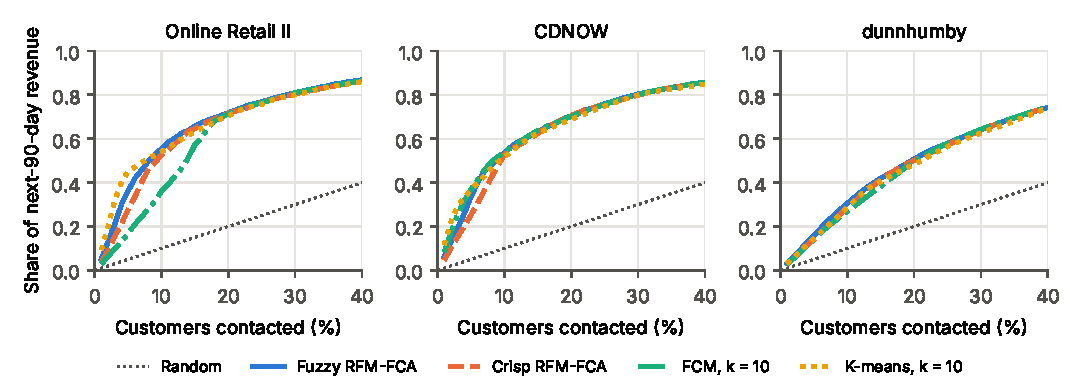
\includegraphics[width=\textwidth]{figures/gain_curves.pdf}
\caption{Cumulative share of next-90-day revenue against the share of customers contacted, ranked by predicted spend (means over four cutoffs).}
\label{fig:gain}
\end{figure}

Table~\ref{tab:targeting} and Figure~\ref{fig:gain} translate predictions into campaign terms. Contacting the top 10\,\% of customers ranked by fuzzy RFM-FCA reaches 0.9--2.9 percentage points more of next-period revenue than ranking by crisp RFM-FCA on every dataset ($p \le 0.01$), the decile where crisp quintile boundaries lump very different spenders together. Fuzzy RFM-FCA reaches more revenue than K-means and GMM at both depths on all datasets; fuzzy C-means is mostly level but fails on the Online Retail II top decile (36.2\,\% vs 55.4\,\%). Of the twelve pre-registered tests at 20\,\% depth (against crisp RFM-FCA and fuzzy C-means, revenue and lift), three are significant, all in favour of fuzzy RFM-FCA. Purchase lift on dunnhumby cannot exceed about 1.08 because almost all households buy, and is uninformative there.

\subsection{Robustness and stability}\label{sec:res-struct}

\begin{table}[t]
\centering\small
\caption{Structural agreement (correlation of customer-pair similarities between a reference fit and a perturbed fit; 1 = identical), mean over 20 replicates. Robustness: 5\,\% of invoices dropped. Stability: bootstrap resample of customers.}
\label{tab:structure}
\begin{tabular}{lcccccc}
\toprule
 & \multicolumn{3}{c}{Robustness} & \multicolumn{3}{c}{Stability} \\
\cmidrule(lr){2-4}\cmidrule(lr){5-7}
Representation & Retail II & CDNOW & dunnhumby & Retail II & CDNOW & dunnhumby \\
\midrule
Crisp RFM-FCA (C-fca) & 0.886 & 0.936 & 0.928 & 0.957 & 0.987 & 0.936 \\
Fuzzy RFM-FCA (F-fca-core) & 0.958 & 0.955 & 0.948 & 0.986 & 0.993 & 0.972 \\
K-means, $k{=}10$ & 0.760 & 0.907 & 0.650 & 0.683 & 0.937 & 0.692 \\
GMM, $k{=}10$ & 0.858 & 0.816 & 0.878 & 0.818 & 0.904 & 0.843 \\
FCM, $k{=}10$ & 0.913 & 0.929 & 0.942 & 0.944 & 0.966 & 0.914 \\
\bottomrule
\end{tabular}
\end{table}


At comparable granularity (Table~\ref{tab:structure}) fuzzy RFM-FCA has the highest mean robustness and stability of all representations on all three datasets. It beats crisp RFM-FCA in 20 of 20 robustness replicates on every dataset, and K-means and GMM in essentially every replicate. Against fuzzy C-means the margin is small and each method wins some replicates, but the worst case of fuzzy RFM-FCA is better in all six dataset--measure cells.

\subsection{Interpretability and the summary view}\label{sec:res-interp}

\begin{table}[t]
\centering\small
\caption{Structural interpretability proxies on the full data (Retail II / CDNOW / dunnhumby). Fidelity: F1 between ``satisfies the segment's R/F/M description'' and ``is a member''. Conditions: constrained dimensions per description.}
\label{tab:interpretability}
\begin{tabular}{lcccc}
\toprule
Representation & Segments & Fidelity (F1) & Conditions & Segments per customer \\
\midrule
Crisp RFM-FCA (C-fca) & 51 / 54 / 49 & 1.00 / 1.00 / 1.00 & 1.5 / 1.6 / 1.5 & 5.3 / 6.2 / 5.5 \\
Fuzzy RFM-FCA (F-fca-core) & 208 / 238 / 215 & 1.00 / 1.00 / 1.00 & 1.8 / 1.9 / 1.8 & 19.5 / 24.0 / 20.9 \\
K-means, $k{=}10$ & 10 / 10 / 10 & 0.68 / 0.74 / 0.74 & 3.0 / 3.0 / 3.0 & 1.0 / 1.0 / 1.0 \\
GMM, $k{=}10$ & 10 / 10 / 10 & 0.53 / 0.80 / 0.67 & 3.0 / 3.0 / 3.0 & 1.0 / 1.0 / 1.0 \\
FCM, $k{=}10$ & 10 / 10 / 10 & 0.66 / 0.71 / 0.73 & 3.0 / 3.0 / 3.0 & 1.0 / 1.0 / 1.0 \\
\bottomrule
\end{tabular}
\end{table}


Table~\ref{tab:interpretability} compares structural proxies. FCA segments are exactly described by their intents (fidelity 1 by construction) in fewer than two conditions on average, whereas the tightest R/F/M description of a cluster disagrees with its membership for 20--47\,\% of customers and constrains all three dimensions. Fuzzy RFM-FCA additionally represents the 74\,\%, 69\,\% and 73\,\% of customers who lie within 0.05 of a quintile cut point on at least one dimension. Its costs are about four times as many segments as crisp FCA (each customer belongs to about 20) and a rule set whose mean confidence is slightly \emph{lower} than the crisp one (0.71 vs 0.73, 0.81 vs 0.84, 0.79 vs 0.81), although individual rules become sharper: on Online Retail II, the crisp rule $\{R5, M5\} \Rightarrow \{R5, F5, M5\}$ has confidence 0.81, while its boundary-aware counterpart $\{R5, M5\} \Rightarrow \{R5, \tfrac12 F5, M5\}$ has 0.92.

\begin{table}[t]
\centering\small
\caption{The 10-concept fuzzy summary of Online Retail II (greedy description-coverage selection, full data). $\tfrac12$X: partly in term X.}
\label{tab:summaryview}
\begin{tabular}{rlrr}
\toprule
\# & Intent & Customers fully in (\%) & Share of spend (\%) \\
\midrule
1 & \{F5, M5\} & 10.3 & 55.3 \\
2 & \{F1, M1\} & 9.9 & 0.4 \\
3 & \{$\tfrac12$F2, $\tfrac12$M2\} & 18.9 & 2.7 \\
4 & \{$\tfrac12$F4, $\tfrac12$M4\} & 18.8 & 13.0 \\
5 & \{$\tfrac12$F3, $\tfrac12$M3\} & 17.9 & 5.6 \\
6 & \{$\tfrac12$F2, M1\} & 4.6 & 0.2 \\
7 & \{F5, $\tfrac12$M4\} & 4.5 & 3.6 \\
8 & \{$\tfrac12$F4, $\tfrac12$F5, $\tfrac12$M5\} & 6.3 & 11.8 \\
9 & \{$\tfrac12$F1, $\tfrac12$M1, $\tfrac12$M2\} & 6.2 & 0.6 \\
10 & \{R5, F5, M5\} & 4.8 & 36.9 \\
\bottomrule
\end{tabular}
\end{table}


The greedy summary addresses the segment count. Table~\ref{tab:summaryview} shows the ten fuzzy segments selected on Online Retail II; they include the high-value groups $\{F5, M5\}$ (10.3\,\% of customers, 55.3\,\% of spend) and $\{R5, F5, M5\}$ (4.8\,\%, 36.9\,\%) and band-straddling groups such as $\{\tfrac12 F4, \tfrac12 F5, \tfrac12 M5\}$. Each customer falls into one or two segments, described by about two conditions. As predictors, the 10-concept fuzzy summary beats the 10-concept crisp summary on all three datasets (AUC $+0.026$, $+0.005$, $+0.016$; $R^2$ $+0.033$, $+0.004$, $+0.011$; Holm $p \le 0.008$) and is far more robust and stable (the crisp summary collapses to a robustness of 0.57 on Online Retail II). Compression has a price: the summary predicts worse than the full lattice and than fuzzy C-means with ten clusters (AUC $-0.005$ to $-0.047$).

\subsection{Sensitivity}\label{sec:res-sens}

\begin{table}[t]
\centering\small
\caption{Sensitivity analysis: number of setting $\times$ dataset $\times$ metric cells in which the fuzzy variant is significantly better (95\,\% interval above zero) and significantly worse. Settings: support 0.02/0.04/0.06, membership half-width 0.15/0.20/0.25, horizon 60/90/180 days.}
\label{tab:sensitivity}
\begin{tabular}{lcc}
\toprule
Comparison & Fuzzy significantly better & Significantly worse \\
\midrule
Fuzzy vs crisp RFM-FCA & 47 / 48 & 0 \\
Fuzzy vs crisp memberships & 29 / 30 & 1 \\
Fuzzy vs crisp summary ($K = 5, 10, 20, 30$) & 18 / 24 & 1 \\
\bottomrule
\end{tabular}
\end{table}


\begin{figure}[t]
\centering
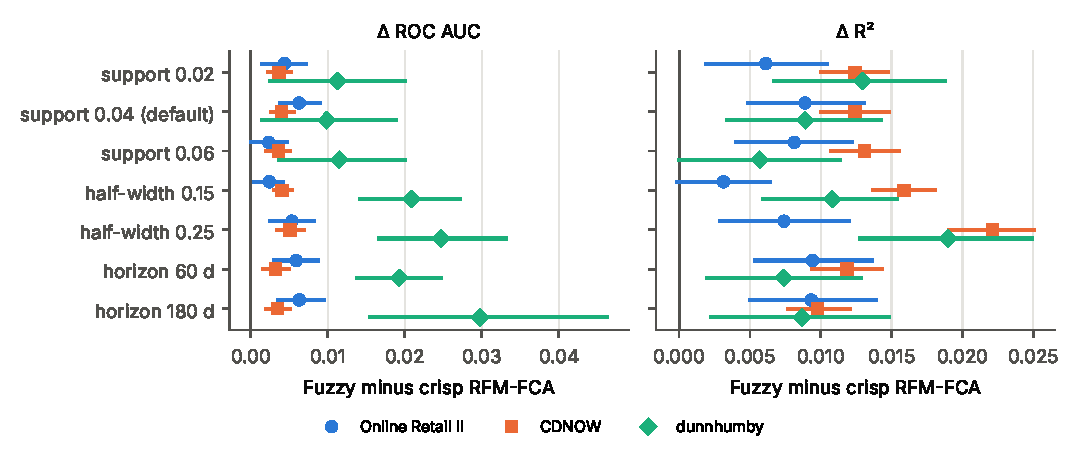
\includegraphics[width=\textwidth]{figures/sensitivity.pdf}
\caption{Difference between fuzzy and crisp RFM-FCA under one-at-a-time parameter changes, with 95\,\% customer-bootstrap intervals.}
\label{fig:sens}
\end{figure}

Every parameter fixed early was varied on all three datasets: the support threshold (0.02, 0.04, 0.06, which changes the number of fuzzy segments from about 140 to about 500), the membership half-width (0.15, 0.20, 0.25) and the horizon (60, 90, 180 days). Fuzzy RFM-FCA is significantly better than crisp RFM-FCA in 47 of 48 cells and never worse (Table~\ref{tab:sensitivity}, Figure~\ref{fig:sens}); the fuzzy-membership result holds in 29 of 30, with one reversal at the narrowest width. For the summary, $K = 10$ is the only size that beats the crisp summary in all six cells.

\subsection{Tie-aware memberships (exploratory)}\label{sec:res-ties}

On CDNOW, the mid-rank places all 11,840 one-time buyers in a single term, and 41 of the fuzzy rules merely restate this tie (e.g.\ $\{\tfrac12 F2\} \Rightarrow \{F2\}$ with confidence 1). The tie-aware membership spreads them over F1--F3, removes all 41 such rules and raises the bootstrap stability of the segment set from 0.908 (worst case 0.524) to 0.963 (worst case 0.920), with unchanged predictions. On the other two datasets it changes at most 0.8\,\% of customers. This was designed after seeing the CDNOW results and is exploratory.
